\newgeometry{textwidth=16cm}
\chapter[4]{Acenes}
\minitoc
\restoregeometry

\newpage

\section*{Introduction}
\markright{INTRODUCTION}{}
\spacing{1.5}

The strategy in the present work is to perform high-precision quantum mechanical calculations based on harmonic (solid state) ahrmonic (gaz phase) electrical and mechanical approximations to compute spectra for individual molecules and dimers. With the anharmonic approach, unscaled computed outcomes including harmonics, overtones, combinations, intermolecular vibrations and other details of spectra can be compared directly with experimental data. The detailed identification of bands in experimental vibration spectra for crude oils and oil fractions may eventually permit the identification of the presence of members of a family of molecules, and the determination of the significance of specific types of molecular interaction arising in these fluids through spectral decomposition. Potential impacts include: improved speciation, and hence fluid characterization; and improved understanding of association phenomena, such as $\pi-\pi$ interactions, and hence transport property prediction. 

Acenes, a family of linear polynuclear aromatic compounds possessing only $\pi-\pi$ interactions, for which high precision experimental data are available up to pentacene \cite{michaelian2012far}, comprise a benchmark example that illustrates both the potential and the computational challenges found in this line of inquiry. In this respect, various calculation hypotheses used for these large molecules are presented, together with the impact of these calculation hypotheses on the quality vis-à-vis experimental data and the computational cost of vibrational spectra. 

Spectral assignments, determined on the basis of both wavenumber and relative intensity values, are made primarily using computed spectra for individual molecules, and dimers. In addition, based on experimental observation assessing the presence of deformed molecules in tetracene and pentacene crystals, impact on vibrational spectra of these deformations is evaluated and the phonon spectra is evaluated for the tetracene system. For some cases, assignment ambiguity is only resolved by tracing trends for vibration modes for the acene family as a whole. In the exposition that follows, each of these topics is tackled sequentially. Calculations with tetracene and pentacene monomers (individual molecules) are treated first. Then calculations for dimers and the acene family collectively are treated, and the results synthesized.

\singlespacing
\section{Calculation of vibrational spectra of Tetracene and Pentacene Monomers: Comparison with experimental data}
\spacing{1.5}
\subsection{Experimental data}

Experimental solid-state infrared spectra of tetracene and pentacene \cite{michaelian2012far} were acquired at room pressure and temperature. The measurements were performed on as received samples. Thus the crystallinity as well as the possible presence of defects in these solids are unknown. For tetracene, two crystal structures have been detected by x-ray diffraction experiments \cite{venuti2004phonons}. At room temperature and pressure, tetracene is triclinic \cite{campbell1962crystal} with space group P\={1}. The unit cell contains two independent molecules at the $(0,0,0)$ and $(1/2,1/2,0)$ inversion sites. Pentacene possesses two polymorphs \cite{venuti2002probing,brillante2005characterization}. One comprises a triclinic layered structure with a herringbone arrangement in the layers, with two equivalent molecules per unit cell \cite{campbell1961crystal}.  The other, commonly found at room temperature, adopts a 14.1 Å d(001)-spacing morphology with an inversion center on both molecules in the unit cell \cite{holmes1999nature,siegrist2001enhanced,mattheus2001polymorphism,mattheus2003identification,mattheus2003modeling}.

\singlespacing
\subsection{Computational details: construction of the potential energy surface}
\spacing{1.5}

The Becke Three-Parameters Hybrid Functional (B3LYP), a combination of the Becke three-parameter exchange functional (B3) \cite{becke1993density} that includes a mixture of Hartree-Fock exchange with the density functional theory (DFT) exchange-correlation and the LYP correlation functional \cite{lee1988development}, has proven to be a reasonable choice for predicting geometries of aromatic molecules \cite{bauschlicher1995comparison,tirado2008performance}.  Stephens et al. \cite{stephens1994ab} showed that the B3LYP force field yields infrared spectra in very good agreement with experimental data. It has become a standard method for studying vibrational spectra of organic molecules (in the far- and mid- Infrared) in the gas phase \cite{bauschlicher1997calculation,gohaud2005vibrational}. Although the B3LYP method coupled with a sufficiently large basis set is a good candidate to study vibrational spectra of polynuclear aromatic molecules \cite{michaelian2012far}, this standard DFT calculation approach fails to describe long-distance interactions. Consequently, it does not reproduce spectra of interacting molecules \cite{becke1993density,stephens1994ab,kristyan1994can,hobza1995density} where the interpretation of experimental vibration spectra requires consideration of both isolated and interacting molecules.

In parallel to the development to ab initio methods, some progress has been made on implementing the London dispersion force effect into DFT methods, permitting calculations with larger individual molecules and binary pairs. Although the CCSD(T) method in combination with a sufficiently flexible basis set is the most accurate method for reproducing rotation-vibration spectra and to describe intermolecular complexes between aromatic hydrocarbons \cite{begue2006new}, such calculations are impractical for the description of large molecules \cite{begue2012nitrile}. The MP2 method \cite{pople1979derivative}, also able to handle dispersive interactions such as $\pi-\pi$ stacking \cite{chalasinski2000state,johnson2006structure},is a computationally intensive and inadequate method for large molecules too \cite{eilmes2012theoretical}. Chai et al.78  developed a functional based on optimized long-range corrected hybrid density functionals \cite{chai2008systematic}, which employs 100\% Hartree-Fock (HF) exchange for long-range electron-electron interactions, $\omega$B97X, to which they added an empirical dispersive interaction correction \cite{eilmes2012theoretica}. This method was tested by Salzner et al \cite{salzner2011improved} for $\pi$-conjugated oligomers and it overcame the difficulties encountered with standard DFT functionals when dealing with interacting $\pi$-systems.

In this work, for isolated molecules and dimers, extended basis-sets consisting of atomic orbitals expressed as fixed linear combinations of Gaussian functions are employed for the calculations.  A split valence 6-311G and 6-311G(p,d) \cite{krishnan1980self,frisch1984self} was needed to provide correct calculation outcomes for naphthalene monomer \cite{saeki2006theoretical}. Validation tests for the $\omega$B97X-D/6-311G calculation method were also performed. The accuracy of DFT calculations in predicting molecular geometries and vibrational frequencies depend on the density functional employed. Thus geometrical optimizations were performed for isolated tetracene, using the $\omega$B97X-D functional as well as the more conventional B3LYP method. The computational results are benchmarked using experimental data obtained by Campbell et al.\cite{campbell1962crystal}

The solid state calculations in the present work were carried out with the use of two approaches:
First, the calculations were carried out with the projector augmented wave (PAW) implementation of Vienna Ab initio Simulation Package (VASP)\cite{kresse1996efficient}. The generalized gradient approximation (GGA) in the PBE parameterization was considered as the exchange correlational functional \cite{perdew1996generalized}. Structural optimizations (triclinic tetracene crystal) were achieved by setting the convergence criteria for total energies are below $5*10^{-6}$ eV, residual forces to be less than $1*10^{-3}$ eV/Å, and stresses limited to 0.02 GPa. To correct the missing dispersion interactions, we have used several recently proposed methods such as PBE functional with pair potential methods D2, D3 (BJ), TS, and TS+SCS. The details of the implementations and usage of these methods can be found elsewhere \cite{grimme2006semiempirical,grimme2011effect,tkatchenko2009accurate,tkatchenko2012accurate,dion2004van}. To obtain accurate band gaps, we have used the GW approximation86.  For getting accurate quasiparticle eigenvalues, we used 200 bands for the summation over the bands in the polarizability and the self-energy formulas, and the polarizability matrices were calculated up to a cutoff  of 200 eV.

Second, periodic calculations for tetracene were also performed in order to calculated IR intensities with CRYSTAL14 program\cite{dovesi2014crystal14}, using PBE functional and STO-6G (Pople's STO-6G) basis set. Default criteria were used as consider accuracy and SCF convergence. Vibrational frequencies at the $\Gamma$ Point were calculated for the optimized geometry. The empirical dispersion correction by Grimme \cite{grimme2006semiempirical} was performed to take into account weak interactions. 

\singlespacing
\subsection{Geometrical parameters of isolated tetracene molecule optimized using B3LYP and $\omega$B97X-D methods associated with 6-311G and 6-311G** basis set}

\spacing{1.5}

Geometry optimizations were performed using two different DFT methods (B3LYP and $\omega$B97X-D) implemented in Gaussian 09 software \cite{frisch2009gaussian}, and two basis sets (6-311G and 6-311G**). While Saeki et al. \cite{saeki2006theoretical}  reported a change of symmetry for the naphthalene molecule, from D2h to C2h (based on MP2/6-311G calculations), optimized geometries for the tetracene molecule, which also possesses D2h symmetry, remained planar with D2h symmetry in all cases. Calculated bond lengths based on different levels of theory are listed in Table 1 along with their mean deviations from experimental measurements (see also Figure A1 in the supplementary data). For these calculations, irrespective of the level of theory or the basis set employed, the agreement between computed bond lengths and experimental values is very good. The mean deviation from experimental values is less than 0.03 Å. These results show clearly that the choice of calculation method and basis set has a minor influence on the geometry of tetracene. Results obtained with pentacene monomer are comparable. This basis-set insensitivity for DFT approaches has been illustrated previously\cite{bauschlicher1995sensitivity}. It permits the use of smaller basis sets and provides an additional argument for the use of DFT over ab initio methods, since larger molecules can be treated. The $\omega$B97X-D method, which contains a London-force dispersive term, and is reliable for acene molecules was selected for this study and it is used in combination with the 6-311G basis-set.

\begin{figure}[H]
	\centering
	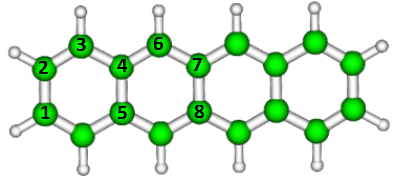
\includegraphics[scale=0.6]{image/tetracene-molecule}\label{tetracene-molecule}
	\caption{Representation of a tetracene molecule.}
\end{figure}

\begin{table}[h]
	\begin{tabular}{c c c c c c c c }
	\toprule
	&$C_{1}-C_{2}$&$C_{2}-C_{3}$&$C_{3}-C_{4}$&$C_{4}-C_{5}$&$C_{5}-C_{6}$&$C_{6}-C_{7}$&$C_{7}-C_{8}$\\
	\midrule
	\multicolumn{1}{p{2.5cm}}{\centering Experimental data$^{a}$} & 1.46 & 1.38 &1.42 &1.42 &1.39& 1.40& 1.46\\
	B3LYP/6-311G& 1.43& 1.36&1.43&1.43&1.40&1.42&1.43 \\
	B3LYP/6-311G**&1.43&1.36&1.43&1.43&1.40&1.42&1.43\\
	$\omega$B97X-D/6-311G& 1.43&1.37&1.44&1.45&1.39&1.41&1.45\\
	$\omega$B97X-D/6-311G**&1.43&1.37&1.44&1.45&1.39&1.41&1.45\\
	\bottomrule
\end{tabular}
\caption{Method and Basis set dependence of C-C bond length (Å) a for tetracene monomer, and mean deviation from experimental data$^{b}$}
\end{table}

\subsection{Truncation of the potential energy surface}

Vibrational spectroscopy modelling outcomes, whether at the harmonic or anharmonic level, are directly dependent on the quality of the potential energy surface (PES). The PES is generally expressed as a polynomial determined by adjustment of a set of geometric structures of a molecule. Consequently this type of calculation depends on the quality of the electronic calculations of the wave functions as well. 
While it is now common to determine the PES accurately for small molecules (3-5 atoms) \cite{begue2007comparison}, this becomes almost infeasible when solving anharmonic approximations for systems of larger size where powerful computers are required to implement rigorous methods for solving the Schrödinger equation. Truncation of the analytical shape of the PES (degree of the potential), is unavoidable. For example, a tetracene molecule contains 30 atoms, and therefore has $3N - 6 = 84$ normal modes apart from the translational and rotational modes. 84 modes with an order 4 necessitates the calculation for 22171 force constants. Thus, truncation of the PES constitutes the first part of this study. Four levels of approximation were tested. The fundamental bands obtained in these cases, using second-order perturbation theory (PT2), are compared to the ones calculated with the complete PES. The conclusion of these tests are summarized in Table 2 and elaborated here:


\begin{enumerate}
	\item It is possible to truncate the PES in terms of only significant coupling. For this, it suffices to identify the constant of cubic and quartic force of very low intensity. We have realized calculations by successively suppressing force constants smaller than 2, 5, 8 and 10 $cm^{-1}$.  This study showed that the discrepancy regarding the calculated frequencies of fundamental modes is not higher than 2.8 $cm^{-1}$, and 3.3 $cm^{-1}$ for the combination modes. These disparities are small enough to justify use of this approximation. Moreover this allows setting 7, 33, 48 and 55 \% of the forces to zero when suppressing constants smaller than 2, 5, 8 and 10 $cm^{-1}$, respectively, thus saving computational cost and enabling variational calculations for larger systems. Note, however, that this restriction is potentially acceptable only without any Fermi or Darling-Dennison resonance, often characterized totally or partially using these finest couplings. Regarding the time saved when suppressing the forces lower than 10 $cm^{-1}$ while the wavenumber values of fundamental modes remain the same, it would be tempting to truncate the PES this way, but this would represent a serious risk of losing information regarding combination bands. Indeed our tests show that the upper limit of the truncation to maintain all the information of combination bands consists in considering all the forces higher than 5 $cm^{-1}$. Removal of these forces would disregard combinations whose weight is less important, resulting in the loss of details that provide a complete interpretation of infrared spectra. Thus, for the following tests of truncature and for calculations presented in this study, we will consider a PES calculated with force constants higher than 5 $cm^{-1}$.
	
	\item The second truncation tested in this work consists of separating modes of high and low wavenumber. We assumed that the description of the low-wavenumber modes (mainly torsion modes), were weakly coupled with bending and scissoring modes occurring at higher wavenumber.  This hypothesis has been tested and validated on the base of calculations on the tetracene molecule (Table 2); indeed each of the first 15 modes calculated using the PES truncated to torsional and libration modes are in perfect adequacy with values calculated a posteriori using complete PES. 
	
	\item We have also tested the association of a complete grid of points of the surface at the fourth order, with a fit at the sixth order on the diagonal, in order to refine coupling between closely coupled modes. Because this refining is demanding in terms of computing time, we applied it on the 10 first modes only, supposing that the modes of higher wavenumber were correctly described with a polynome of $4^{th}$ order. The results, listed in Table 2, show that this refining doesn’t bring any improvement for describing the vibrational spectrum of tetracene.
	
	\item The last approximation used in this work consists of applying a second adjustment of the PES; this adjustment would aim to eliminate the weight of vibrators we excluded in point (i), to refine the fit of remaining force constants so that they reflect, in fine, only the couplings between remaining modes. If this had proved to be an acceptable approximation, we could have extended this methodology to the study of specific molecules vibrators of undifferentiated dimension, by calculating a limited number of specific points to sought vibrators. In accordance with what Bowman et al \cite{bowman2008variational} and Begue et al \cite{begue2010calculation}  showed on the study of water clusters, our calculations show that only the separation between libration modes with all other active modes is possible.
	
\end{enumerate}

To conclude, we have shown that partial truncation of PES could be effective for our study. This truncation consists of extracting from a global fit, the force constants of higher order that allow the description of the problem beyond the harmonic approximation. These constants can then be directly used to solve Schr\"{o}dinger's vibrational equation.

This methodology was used in the remainder of our work for the characterization and assignment of the spectra of tetracene and pentacene molecules.

\begin{table}[htb]
	\caption{Force constant truncation and separation of low and high mode influences on the values of wavenumbers of tetracene monomer based on a force field extracted from calculations at the $\omega$B97X-D/6-311G level of theory. }
	\begin{center}
		\begin{tabular}{c c c c c c c c}
			\toprule
			\multicolumn{1}{p{2.5cm}}{\centering Polynomial \\ degree} &  & 2 & 4$^{c}$ & 4$^{c}$ & 4$^{c}$ & 4$^{c}$ & 6$^{c}$\\
			\multicolumn{1}{p{2.7cm}}{\centering Force constants \\ (f) considered} &  &  & \multicolumn{1}{p{2cm}}{\centering All f \\ considered} & f>5cm$^{-1}$ & f>5cm$^{-1}$ & f>5cm$^{-1}$ & \multicolumn{1}{p{2cm}}{\centering All f \\ considered} \\
			\multicolumn{1}{p{2.5cm}}{\centering Number of \\ modes}& & 84  & 84  & 84  &	20  &	10 & 10 \\
			\multicolumn{1}{p{2.5cm}}{\centering Mode \\ (symmetry)} & Exp. values$^{a}$ &  &  &  &  &  & \\
			\midrule
			$\nu_{1}(B_{3u})$ &  & 57 & 48 & 53 & 62 & 	60 & 69 \\
			$\nu_{2}(A_{u})$ &  &  93 & 90 & 96 & 107 & 103 & 107\\
			$\nu_{3}(B_{1g})$ & & 154 & 150 & 154 & 161 & 160 & 164\\
			$\nu_{4}(B_{1u})$ & 166$^{b}$ & 168 & 169 & 160 & 169 & 169 & 171\\
			$\nu_{5}(B_{2g})$ &  & 196 & 194 & 200 & 204 & 202 & 203\\
			$\nu_{6}(B_{3u})$ & 271$^{b}$ & 276 & 272 & 277 & 284 & 282 & 284\\
			$\nu_{7}(B_{3g})$ & & 316 & 317 & 305 & 317 & 317 & 319\\
			$\nu_{8}(A_{g})$ & 322$^{b}$ & 324 & 322 & 323 & 322 & 320 & 322\\
			$\nu_{9}(A_{u})$ &  & 327 & 325 & 332 & 330 & 328 & 331\\
			$\nu_{10}(B_{1g})$ &  & 389 & 382 & 386 & 395 & 392 & 394\\
		\bottomrule	
		\end{tabular}
	\end{center}
	\footnotemark{a Experimental values of wavenumbers are obtained from \cite{michaelian2012far}.}
	\footnotemark{b Experimental uncertainty equal to +/- 2 cm$^{-1}$.}
	\footnotemark{c Wavenumbers calculated using second-order perturbation theory (PT2).}
\end{table}


\singlespacing
\subsection{Resolution of the vibrational Schrödinger equation (non-core bands with intensity)}

\spacing{1.5}

 The presence of overtones and combination bands in infrared spectra is a manifestation of the breakdown of the double-harmonic approximation, usually implemented in electronic structure codes. The calculation of intensities is essential in order to determine which non-fundamental transitions are active and to assign all experimental bands. Since both mechanical (anharmonicity of the potential) and electrical (non-linear dependence of the dipole moment on the normal coordinates) anharmonicities are expected to give non-zero intensities to non-fundamental transitions, these two effects must be considered in the treatment of transition energies and related vibrational wavefunctions. The wavenumber calculations in the mechanical anharmonic approximation were carried out using a variational method developed by Bégué et al \cite{begue2007comparison} Using this method, implemented in the P\textunderscore Anhar.v2.0 program \cite{gohaud2005new},  it was possible to compute all the vibrational frequencies (fundamental, combination bands and overtones) that contribute to the mid- and near-infrared spectrum of tetracene and pentacene. In addition, the activity of each mode was also calculated in the electrical anharmonic approximation using a method developed by Baraille et al \cite{begue2010calculation,baraille2001calculation} , which is also available in the same software.

The experimental spectra of tetracene and pentacene, extracted from the work of Michaelian et al \cite{michaelian2012far} , are shown in Figure 2. The corresponding calculated infrared active transitions both fundamental and combination bands overlay the data and are listed in Table 3 and Table 4 where they are further compared with available experimental and theoretical values. Threshold intensity for IR-activity of 0.001 km/mol was chosen for the calculations. This threshold is justified following a discussion of band assignments for each molecule, and presentation of vibrational bands common for the two molecules.

\begin{figure}[h]
	\centering
	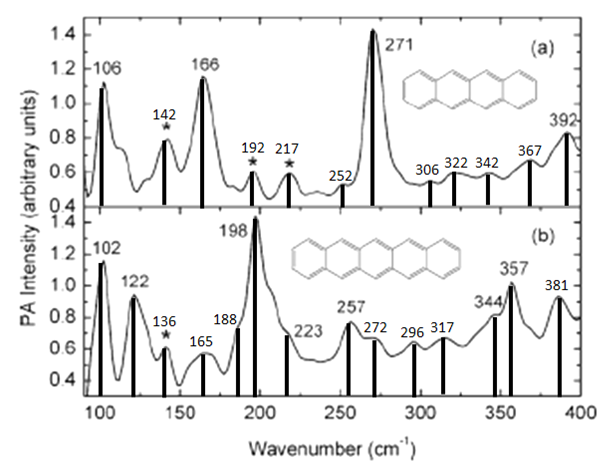
\includegraphics[scale=0.8]{image/spectra-TP}
	\caption[Far-infrared PA spectra of (a) tetracene; (b) pentacene]{Far-infrared PA spectra of (a) tetracene; (b) pentacene. Spectra were acquired using phase modulation at a frequency of 5 Hz and an amplitude of 15 $\lambda$ ($\lambda = 0.6328 \mu m$), extracted from Michaelian et al \cite{michaelian2012far} } \label{spectra-TP}
\end{figure}

\begin{table}[htb]
	\caption{Experimental and calculated wavenumbers (cm-1) for fundamental and combination vibrational modes of tetracene.}
	
	\begin{center}
		\resizebox{18cm}{!}{
		\begin{tabular}{c c c c c c c c c}
			\toprule
			 &  &  & \multicolumn{1}{p{2cm}}{\centering Experimental \\ values} & \multicolumn{5}{p{12cm}}{\centering Predicted bands}\\
			 \textbf{Mode} & \multicolumn{1}{p{1.8cm}}{\centering \textbf{Type of} \\ \textbf{vibration}} & \textbf{Symmetry} & \multicolumn{1}{p{1.8cm}}{\centering \textbf{Michaelian} \\ \textbf{et al\cite{michaelian2012far}}} & \multicolumn{1}{p{1.8cm}}{\centering \textbf{Michaelian} \\ \textbf{et al\cite{michaelian2012far}}} & \multicolumn{1}{p{1.8cm}}{\centering\textbf{Cataldo}  \\ \textbf{et al\cite{cataldo2013far}}} & \multicolumn{1}{p{1.8cm}}{\centering \textbf{Harmonic} \\ \textbf{cm$^{-1}$}} & \multicolumn{1}{p{1.9cm}}{\centering \textbf{Anharm} \\ \textbf{(PT2) cm$^{-1}$}} & \multicolumn{1}{p{1.9cm}}{\centering \textbf{Theoretical IR} \\ \textbf{Intensity$^{a}$ km/mol}}\\
			\bottomrule	
		\end{tabular}}
	\end{center}
\end{table}


For tetracene molecules, three bands were identified previously in the range 100 – 400 cm$^{-1}$ \cite{michaelian2012far,malloci2007time}. Two were noted as infrared active at 166 and 271 cm$^{-1}$, and one (388 cm$^{-1}$) was assigned as Raman-active (Table 3). By calculating intensities for all bands, including combination bands and overtones, 8 additional infrared- active vibrations (7 combinations and one second-harmonic) are identified, and the band at 388 cm$^{-1}$ previously assigned as Raman-active is identified as an infrared-active band arising from the B3u mode plus an overtone. Three similar cases where a vibrational transition could correspond either to a  combination band, an overtone, or a Raman-active band, are also shown in Table 3.

\subsection*{Raman-transition active in infrared: molecular deformation}

Raman transitions can become active in infrared spectre, when a molecule is deformed in the solid state. For example, Homes et al.58 showed experimentally that acene molecules in the solid state are not planar and attributed this observation to crystal-packing forces that induce deformation; additionally, deformation effect on lattice-phonon frequencies has been measured, then enabling discrimination of different solid phases of tetracene \cite{venuti2004phonons} and pentacene \cite{venuti2002probing,brillante2002raman}. 
In order to underpin this contention, we performed calculations on a deformed tetracene molecule, shown in Figure 3. In this conformation the molecule does not possess D2h symmetry. The molecule does still possess symmetry, however. The deformation concerns dihedral angles [C1-C2-C3-C4], [C2-C3-C4-C5], [C4-C5-C6-C7], [C5-C6-C7-C8], [C9-C10-C11-C12] and [C10-C11-C12-C13], equal to 175$^{\circ}$ , 178$^{\circ}$ , -178$^{\circ}$, -178$^{\circ}$, -178$^{\circ}$, -178$^{\circ}$, respectively, instead of $\pm$180$^{\circ}$ in the case of the molecule in the D2h conformation. The bond lengths are unchanged. Wavenumbers of fundamental modes and associated intensities calculated with the harmonic approximation are listed in Table A1 in the supplementary data. The calculated vibrational spectrum exhibits only positive wavenumbers, which attests that this deformation is located at a minimum of the PES. The intensities corresponding to the R-denominated-bands of the deformed molecule, calculated at the harmonic level, are given in Table 3. For the deformed molecule, modes that would normally be inactive in infrared (Raman active or silent modes), present significant intensities, ranging from 0.002 to 0.05 km/mol.

\begin{figure}[h]
	\centering
	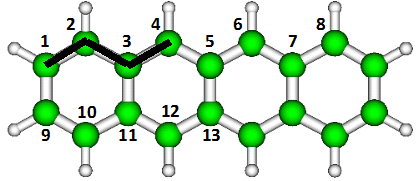
\includegraphics[scale=0.6]{image/Tetracene-def}
	\caption[The deformed dihedral angle C1-C2-C3-C4 in Tetracene molecule]{Tetracene molecule. The deformed dihedral angle C1-C2-C3-C4 is shown in black.}
\end{figure}

\subsection*{Assignment based on intensity value}

Transitions for which there is a double hypothesis (142, 192 and 392 cm$^{-1}$) can be resolved on the basis of relative intensity values. Thus the band at 142 cm$^{-1}$ could be attributed to a second harmonic whose intensity would be three times lower than the Raman-active one that becomes optically active for the deformed molecule. The band at 192 cm-1 could be either a combination of an IR-active mode and a Raman-active mode, whose intensity would be ten times lower than a Raman-active band calculated at 196 cm$^{-1}$. The band at 392 cm$^{-1}$ could either be a combination of an overtone and an infrared active mode, or a Raman-active band ten times more intense. From the relative intensities, in each case, the assumption of the Raman-band becoming active is more likely. For other transitions, there is a single hypothesis. The transition, denoted v$_{8}$, located at 322 cm$^{-1}$ is a Raman-active band while the bands located at 252, 306 and 342 cm$^{-1}$ are combination bands. 

For pentacene, Table 4, the situation is similar. 11 bands arise from combination vibrations. One, found experimentally at 257 cm$^{-1}$, was previously assigned to a predicted Raman-active mode. Calculations on a deformed pentacene molecule lead to an IR active band at a comparable wavenumber and with a comparable intensity. Thus, this one assignment remains uncertain on the basis of these calculations. 

\subsection*{Use of trends for assignment}

The trends for normal modes of infrared active vibrations found for both tetracene and pentacene molecules (see types of vibration in Table 3 and Table 4) are shown in Figure 4 where they are also compared with experimental data. By viewing the wavenumbers in this way, wavenumber assignments for the two molecules can be evaluated in parallel. From the similarity of the trends for tetracene and pentacene, as well as the proximity of the respective computed wavenumbers to experimental ones, the assignment choices - combination bands over Raman-active ones – are supported and this outcome is independent of intensity values. Only one band remains unassigned in the experimental spectrum of tetracene, 106 cm-1. Michaelian et al \cite{michaelian2012far} suggested that it originated from lattice vibration. The pentacene band attributed to a Raman-active vibration, 102 cm$^{-1}$, may be of the same type as well.  These bands and intermolecular bands more broadly are addressed by performing calculations with tetracene and pentacene dimers. 

\begin{figure}
	\centering
	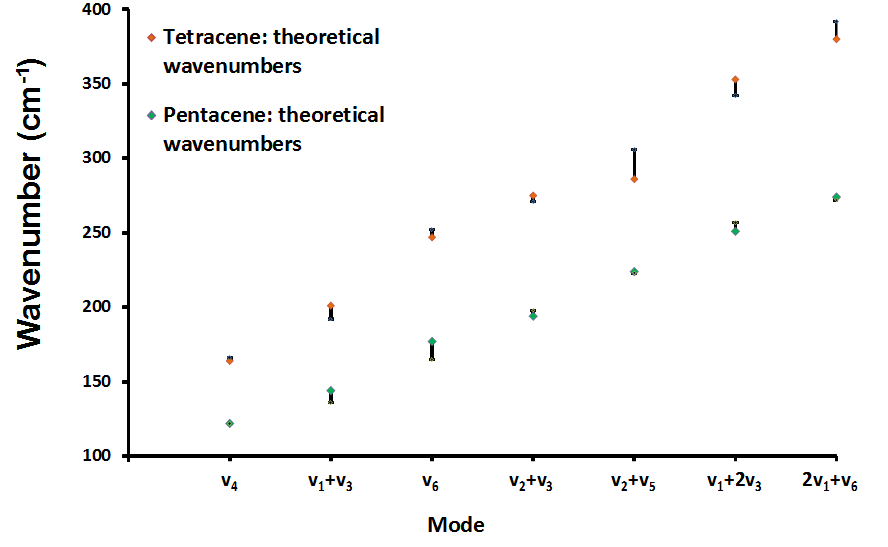
\includegraphics[scale=0.6]{image/comparison}
	\caption[Comparison of theoretical and experimental wavenumbers of tetracene and pentacene]{Comparison of theoretical and experimental wavenumbers of tetracene and pentacene for the same normal modes of vibration. The deviations between experimental and theoretical wavenumbers are represented with dark bars.}
\end{figure}

\singlespacing
\section{Calculation of vibrational spectra of acene dimers: Comparison with experimental data.}
\spacing{1.5}


$\Pi$-stacking is responsible for the cohesive structure of acene crystals \cite{campbell1962crystal,mattheus2001polymorphism,brock1982temperature,facelli1993determination,brock1990temperature}. Dimers constitute a benchmark for describing $\pi$-stacking phenomena. In order to generalize the effect of $\pi$-stacking on intermolecular vibrations for the acene family as a whole, the calculations described here include those for naphthalene and anthracene dimers in addition to the tetracene and pentacene dimers. Inclusion of these smaller dimers also permits calibration of the computational methodology employed.  

\singlespacing
\subsection{Calculated geometry and wavenumbers of dimers and comparison with experimental data}
\spacing{1.5}


Far-infrared spectra provide information about intermolecular and inter-ring interactions and about $\pi$-stacking in particular. Hineno et al \cite{hineno1975far}  measured spectra of naphthalene and anthracene in the region 190-50 cm$^{-1}$ at liquid helium temperature and observed that some bands were due to lattice vibrations. In the same way, bands in the experimental vibrational spectra of tetracene and pentacene that cannot be interpreted based on computed wavenumbers for a single molecule are expected to arise from lattice modes. A first step toward understanding $\pi -\pi$ interaction of acene compounds consists of considering the interaction of acene dimers. The choice of the calculation method for describing these electronic interactions is justified, and then the differentiation of inter- and intramolecular vibrations in the acene family, is addressed.\\

\textbf{Naphthalene dimer}: to assess the performance of the $\omega$B97X-D method for $\pi -\pi$ interaction calculations involving aromatic molecules, the robustness of the $\omega$B97X-D/6-311G method for naphthalene dimers, for which a broad literature exists \cite{saeki2006theoretical,brillante2002raman} 50,97,98,99,100, is discussed in light of results based on reliable data and accurate computational results. For example, Gonzalez et al.102 and Tsuzuki et al \cite{tsuzuki2004high} calculated ground-state structures and binding energies of van der Waals dimers of naphthalene using an aromatic intermolecular interaction model, at the MP2 and CCSD(T) levels of theory, respectively, using Pople’s basis sets of various size. Their calculations yield two low energy dimers of similar energy: D$_{2d}$ (crossed) and C$_{2h}$ (parallel-displaced), and two C$_{2v}$ T-shaped structures. Walsh et al \cite{walsh2002ab,rubevs2008investigation}, using calculations at the MP2/6-31*(0.25) level found eight stationary points for naphthalene dimers: the four reported previously and four others of lower symmetry. Following these studies, Saeki et al \cite{saeki2006theoretical} performed vibrational analysis of naphthalene dimers at the MP2/6-311G level of theory and their results are compared with the values obtained in this work. 
In the present work, geometry optimizations of naphthalene dimers in various configurations - parallel displaced (PD), parallel displaced according to C$_{2h}$ symmetry, crossed-parallel according to C$_{2}$ and D$_{2h}$ symmetry - using the $\omega$B97X-D method, with the 6-311G and 6-311G(p,d) basis sets were performed. All stationary points were characterized by frequency calculations to ensure that the optimized structures were located at a local minimum. The basis set superposition error (BSSE) correction developed by Simon et al.106 was included in the calculations for all complexes. Calculations without this correction were carried out to characterize the importance of this error. Negative binding energies indicate exothermic complex formation \cite{boys2002calculation}. Analysis of dimer configurations showed that only the low-level symmetry configurations, C$_{2}$ and parallel-displaced (PD), represented in Figures 5a and b, respectively, correspond to minima on the PES. Vibrational calculations for the symmetric configurations exhibited negative frequencies. This outcome is in agreement with Walsh et al \cite{walsh2002ab} who showed that structures of low symmetry are the most stable. The center of mass separation (r), rotation angle ($\Theta$) for the C2 structure, and the distance of relative translation (x1 and x2) for the PD structure are given in Table 5. For these two configurations the interaction energies at the different levels of theory considered, with and without BSSE correction, as well as the first harmonics, are reported in Table 6. Interaction energies and associated wavenumbers were obtained using $\omega$B97X-D and 6-311G, 6-311G** and cc-pVDZ basis sets. Computed values are compared with results obtained by Walsh et al \cite{walsh2002ab}, Saeki et al \cite{saeki2006theoretical} and Rubes et al \cite{rubevs2008investigation}. BSSE-correction lowers the absolute value of the energy by 1.5 kcal.mol-1 on average, and represents only 0.04\% of the binding energy.  Thus BSSE-correction does not affect the order of stability of the tested configurations. This outcome is in full agreement with the cited prior work. Further there are no trends for the impact of basis-set and BSSE-correction on the geometry of the dimer configurations. However, by calculating the mean difference of computed values, this work, with those of Saeki et al \cite{saeki2006theoretical} shows the  6-311G basis-set combined with BSSE-correctionto be a preferred option.

\begin{figure}[h]
	\centering
	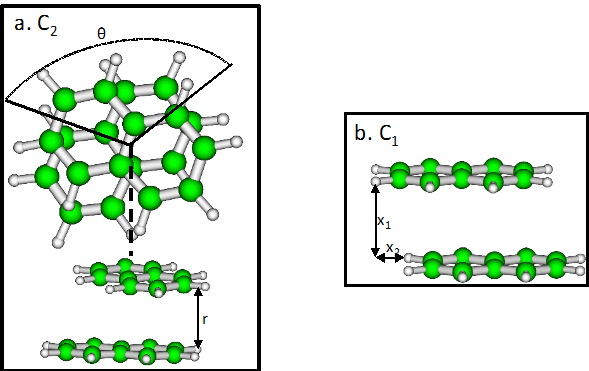
\includegraphics[scale=0.7]{image/napthalene-dimer}
	\caption[Optimized geometries for naphthalene dimers]{Optimized geometries at the $\omega$B97X-D/6-311G level of theory for naphthalene dimers in the most stable configurations a) C2, and b) Parallel-displaced (PD)}
\end{figure}

\textbf{Vibration modes of naphthalene dimers}: Wavenumber calculations for stable dimers were performed using the $\omega$B97X-D/6-311G method with BSSE correction. From vibrational analysis of the monomer (Table A2 in the supplementary data) and the dimer (Table 7) the vibrational modes arising from intra- and intermolecular modes can be discriminated. The assignments are reported in Table 7 for sets of calculations performed as part of this work and from Saeki et al\cite{saeki2006theoretical}. Calculated values are compared with experimental data when available. The calculations were performed with counterpoise correction for both the C2 and PD configurations. The calculated intra- and intermolecular wavenumbers, irrespective of calculation details, are readily distinguished for naphthalene. The intermolecular wavenumbers are at $\sim$100 cm$^{-1}$ and lower, while the intramolecular wavenumbers are greater than $\sim$100 cm$^{-1}$.

\subsection{Pi-stacking in the acene family}

Optimization at the $\omega$B97XD/6-311G level with BSSE correction gives rise to the expected parallel tilted configuration \cite{brock1990temperature} for anthracene, tetracene and pentacene dimers, as shown in Figure 6. This configuration closely resembles that found in triclinic tetracene\cite{campbell1962crystal} and pentacene\cite{holmes1999nature} crystals. The associated interaction energies are reported Table 8.  Other configurations were found to be unstable. They possess negative calculated harmonic values and were clearly not located at a minimum of the PES. So, only naphthalene has a more energetically stable C$_{2}$ configuration. Computations related to both the C$_{2}$ and PD configurations for naphthalene are shown in Table 7. The PD configuration results are used for comparisons with other acene family members where it is the most stable configuration.
For a given geometry, in this case parallel-tilted, the binding interaction energy increases with the number of interacting cycles in a non-linear manner. This result is consistent with previous studies by Hohenstein et al \cite{hohenstein2010density} and Grimme et al\cite{grimme2008special} who compared interaction energies of naphthenic and aromatic dimers of increasing size using the B2PLYP/TZV(2d,p) level of theory. They found that arene dimers were strongly preferred over equivalent naphthenic dimers, especially for anthracene and tetracene, which were stabilized by 3 to 4 kcal.mol$^{-1}$. The calculations reported here are in accordance with these prior results and confirm the prevalence of $\pi$-stacking interactions.  

The wavenumbers assigned to intermolecular (Table 9) and intramolecular (Table 10) modes of vibration for the acene family were calculated at the $\pi$B97XD/6-311G level of theory using BSSE correction. The characteristic wavenumbers for intermolecular vibrations fall in the same range for all  acene dimers. The lower bound wavenumbers are 15 - 33 cm$^{-1}$ and the upper bound wavenumbers are 94 - 112 cm$^{-1}$. The wavenumbers for the intramolecular vibrations are found at higher wavenumbers but begin to overlap with the intermolecular vibration wavenumbers starting with anthracene where the intermolecular mode at a wavenumber of 111 cm$^{-1}$ with an intensity of 0.8 is not readily discriminated from the intramolecular mode at 112 cm$^{-1}$ with an intensity of 1.2, on the basis of wavenumber or intensity value. Thus, inter and intramolecular vibrations are easily discriminated for naphthalene, and the inter- and intramolecular vibration modes are uncorrelated. For anthracene, tetracene and pentacene, the lowest intramolecular vibration modes fall within the range of intermolecular vibrations. 

Four vibration modes, given in Table 9, corresponding to rotation, translation, rotation of the dimer combined with translation and rotation movements of one molecule relative to the other, are common for all four dimers. The last two intermolecular modes are compound-specific. For tetracene, the two additional modes comprise twisting movements of molecular pairs in the same (87 cm$^{-1}$) and in the opposite direction (112 cm$^{-1}$). For pentacene, one is a wagging movement (74 cm$^{-1}$) and the other comprises an opposite direction wagging movement combined with vertical translation normal to the two molecules (95 cm$^{-1}$). For anthracene, one mode is a rotation of one molecule relative to the other, and the second is split into two modes. These latter two modes, at 111 and 112 cm$^{-1}$, consist of a butterfly movement by one molecule with a half-twisting movement by the other simultaneously.

The other vibration modes, shown in Table 10 correspond to intramolecular vibrations. For every type of vibration, simultaneous vibration of each molecule is observed, either in the same or opposite direction, resulting in two wavenumbers. These alternating motions are characterized by wavenumbers and intensities that depend on the value of the dipole moment. The butterfly vibration mode presents very different wavenumbers depending on whether the molecular movements are in the same or opposite direction. Differences range in value from 8 to 42 cm$^{-1}$. The impact of relative movement increases with the number of aromatic rings, due to the correlation with twisting modes at higher frequencies. 

\begin{figure}[h]
	\centering
	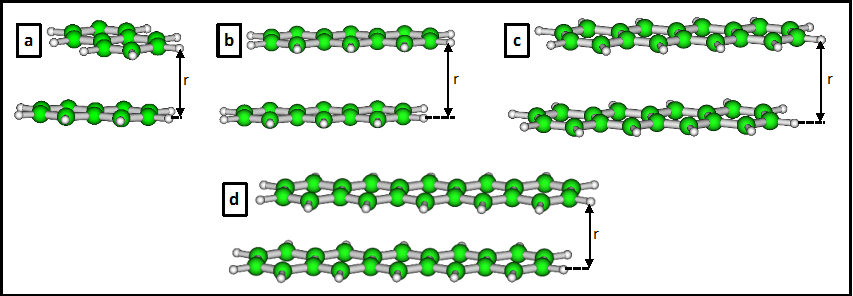
\includegraphics[scale=0.55]{image/acene-dimers}
	\caption[Acene dimers in the parallel displaced configuration]{Acene dimers in the parallel displaced (PD) configuration: a) naphthalene, b) anthracene, c) tetracene, d) pentacene}
\end{figure}

\textbf{Trends in values for specific bands in the acene family}: In order to visualize the effect of the number of aromatic rings on the wavenumbers of specific vibration modes, intramolecular vibration modes and intermolecular vibrations are presented in Figure 7 and Figure 8, respectively. Intramolecular vibration modes, shift to lower wavenumbers with increasing molecule size irrespective of the vibrational mode considered, as was observed for monomers. Butterfly (B), Twisting ($\tau$), Wagging ($\omega$), Stretching ($\sigma$), and Rocking ($\rho$) movements behave similarly. By contrast, the intermolecular vibration modes, found at similar wavenumbers for all the molecules in the acene family, appear specific to this family, and may be used as a reliable fingerprint. In addition, twisting vibration bands appear for dimers of tetracene at (208 cm$^{-1}$) and pentacene at (168 cm$^{-1}$) that replace corresponding twisting bands for monomers at 154 and 104 cm$^{-1}$. The absence of a mode at 154 cm$^{-1}$ for tetracene dimers supports the hypothesis that the feature observed experimentally at 142 cm$^{-1}$ for monomers (see Table 3) is an overtone.

\begin{figure}[h]
	\centering
	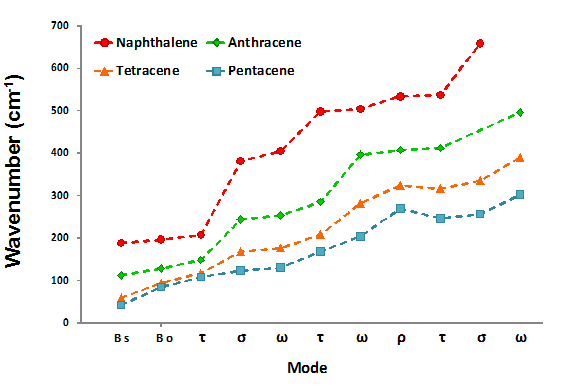
\includegraphics[scale=0.85]{image/intramolecular-v}
	\caption[Comparison of theoretical intramolecular vibration modes for acenes dimers]{Comparison of theoretical intramolecular vibration modes for naphtalene, anthracene, tetracene and pentacene dimers: B s and B o designate butterfly modes, same (s) and opposite (o) direction respectively; $\tau, \sigma, \omega$, and $\rho$ take place for twisting, stretching, wagging and rocking modes respectively}
\end{figure}

\begin{figure}[h]
	\centering
	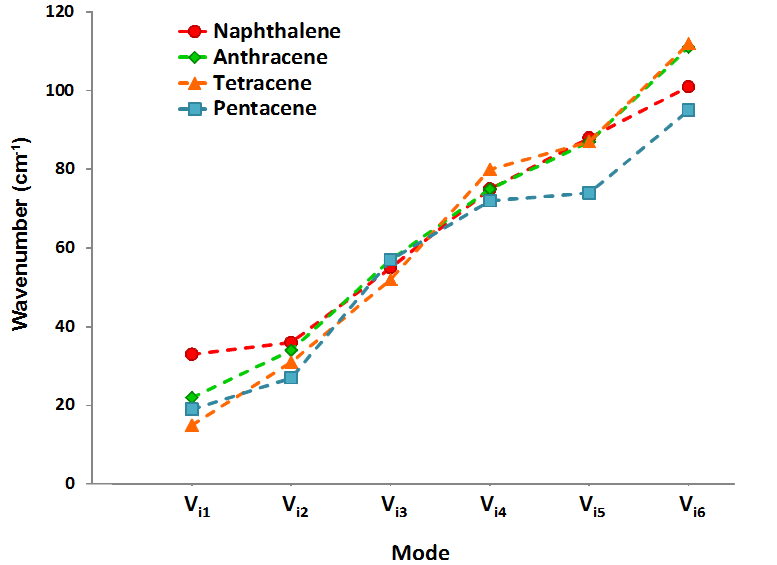
\includegraphics[scale=0.75]{image/intermolecular-v}
	\caption[Comparison of theoretical intermolecular vibration modes for acenes dimers]{Comparison of theoretical intermolecular vibration modes for naphthalene, anthracene, tetracene and pentacene dimers}
\end{figure}

\subsection{The impact of molecule distortion on the vibration modes of acene dimers}

The impact of molecular distortion on vibration modes for dimers was evaluated in the same manner as for monomers. The molecular conformations were perturbed as illustrated in Figure 3 and the distance r (defined in Figure 6) between the molecules was set equal to 3.4, 3.4 and 2.9 Å for naphthalene, anthracene and tetracene dimers, respectively.  As distortion reduces the aromaticity of the molecules, the stability of $\pi$-stacked dimers is expected to be reduced or eliminated. Table 11, where interaction energies for these systems are listed, highlights this loss of stability. For example, no conformations for distorted pentacene dimers correspond to local minima in the PES. Distortion did not affect intramolecular modes of vibration overall for dimers as shown in Table A3 in the supplementary data. Only butterfly vibration modes for anthracene and tetracene, whose wavenumbers get closer to the ones observed for monomers, shown in Table 10, appear to be affected. Some other modes, for which two wavenumbers are given in Table A3, do not exhibit the combined movement of the two molecules either in the same direction or in the opposite direction (as observed for the other intramolecular modes), but movement of the molecules simultaneously. These exceptions are a consequence of the decoupling between the molecules forming the distorted dimer. However, the intermolecular vibration modes, shown in Table 12, are shifted to lower wavenumbers compared to the symmetric analogues shown in Table 9. For the symmetric dimers, the intermolecular vibration modes are effectively independent of molecule size, while for the distorted molecules, the vibration modes tend to lower values as molecular size increases. 
The behavior of the symmetric dimers is attributed to a balancing of opposing effects. One would expect intermolecular vibration modes to shift to lower wavenumbers with increasing ring number (as is observed for intramolecular modes). However, the intensity of the intermolecular interactions increases with the number of rings (Table 8) for symmetric dimers, and this tends to increase wavenumbers. This compensative effect is diminished or absent for the distorted dimers, hence the difference in behavior, and wavenumber invariance for a given intermolecular vibration mode may be a characteristic of $\pi$-stacking interactions. 

\singlespacing
\subsection{Identification of unassigned peaks in the experimental spectra of tetracene and pentacene}

\spacing{1.5}

 By subtracting the intermolecular wavenumbers from the symmetric dimer vibrational spectra of tetracene and pentacene, and comparing the resultant spectra with the spectra of the corresponding monomers, there are two peaks, one for tetracene at 117 cm$^{-1}$ and one for pentacene at 108 cm$^{-1}$, with intensities in the same order of magnitude as the ones calculated for fundamental bands for tetracene (0.34 km/mol) and pentacene (0.15 km/mol). These peaks arise because for every vibrational mode occurring for monomers, there are two quasi-degenerate modes arising for dimers depending on whether the molecules vibrate in the same or in the opposite direction. Thus modes that are Raman-active for a monomer become infrared-active for dimers vibrating in the opposite direction. 
 
 With this final set of assignments, the inter- and intramolecular vibration analysis for the acene family of compounds is complete. Figure 9 gives a direct comparison of experimental and calculated spectra with our conclusion as for assignment. There are no residual unassigned peaks in the available experimental spectra and ultra low wavenumber intermolecular peaks are hypothesized.  While these have yet to be measured experimentally, identification and discrimination of inter- and intramolecular bands at low wavenumbers will play a more important role in the future as the range of IR measurements broadens. For example, by using coherent synchrotron radiation it is becoming possible to make experimental photoacoustic IR measurements in the range 7 to 30 cm$^{-1}$ as demonstrated recently by Billinghurst and Michaelian\cite{billinghurst2010photoacoustic}. DFT calculations have much to contribute to this development, and the interpretation of results obtained.
 
 
 \begin{table}[htb]
 	\caption{Intermolecular distance and Interaction energies calculated for acene dimers.}
 	\begin{center}
 		\begin{tabular}{c c c c c}
 			\toprule
 			textbf{Dimers} & \textbf{Naphthalene} & \textbf{Anthracene} & \textbf{Tetracene} & \textbf{Pentacene}\\
 			\midrule
 			Intermolecular distance r(\AA) & 3.41 &3.27 & 2.96 & 2.98 \\
 		 	 $\omega$B97XD/6-311G + &  & & & \\
 		 	 BSSE corection & -7.53 & -11.52 & -15.73 & -20.44\\
 		 	 Hohenstein et al\cite{hohenstein2010density} & & & & \\
 		 	 SAPT0/aug-cc-pVDZ &-7.27 &  	-12.24 & -17.49 & -22.91\\ 
 		 	 \bottomrule		 		 				
 		\end{tabular}
 	\end{center}
 \end{table}
 
 \begin{table}[htb]
 	\caption{Calculated intermolecular vibrational modes (cm$^{-1}$) and their intensities for naphthalene, anthracene, tetracene and pentacene dimers.}
 	\begin{center}
 		\begin{tabular}{c c c c c}
 			\toprule
 			\textbf{Type*} & \textbf{Naphthalene} & \textbf{Anthracene} & \textbf{Tetracene} & \textbf{Pentacene}\\
 			\midrule
 			Rotation 1/2 & 33(0.04) & 22(0.004) & 15(0.002) & 19(0.002)\\
 			Translation 1/2 & 36(0) & 34(0) & 31(0) & 27(0)\\
 			\multicolumn{1}{p{4cm}}{\centering Total rotation + \\ Translation 1/2 } & 		55(0) & 57(0) & 52(0) & 57(0)\\
 			 & 75(0.21) &  75(0.05) &  87(0.14) &  74(0.07)\\
 			 Rotation 1/2 & 88(0.08) &  87(0.8) & 80(0.96) & 72(0.9)\\
 			  & 101(0) &  111(0.8)/112(1.2) &  112(0) &  95(0)\\
 			  \bottomrule
 		\end{tabular}
 	\end{center}
 	\footnotemark{1/2 means one molecule relative to the other one}
 \end{table}
 
 
 \begin{table}[htb]
 	\caption{Intramolecular vibration modes (cm$^{-1}$) and the corresponding intensities in brackets (km/mol) for naphthalene, anthracene, tetracene and pentacene dimers. Values of corresponding monomer modes are written below in italics.}
 	\centering    
 	\begin{tabular}{c c c c c}
 		\hline 		
 		\textbf{Type*} & \textbf{Naphthalene} & \textbf{Anthracene} & \textbf{Tetracene} & \textbf{Pentacene}\\
 		\hline
 		\multicolumn{1}{p{3cm}|}{Butterfly sw} & \multicolumn{1}{p{3cm}}{\centering 188(3.8) \\ \textit{177(3.2)}} & \multicolumn{1}{p{3cm}}{\centering 111(0.8)/112(1.2) \\ \textit{93(1.5)}} & \multicolumn{1}{p{3cm}}{\centering 59(0.6) \\ \textit{57(0.8)}} & \multicolumn{1}{p{3cm}}{\centering 42(0.4) \\ \textit{38(0.5)}} \\
 		\multicolumn{1}{p{3cm}|}{Butterfly ow} & \multicolumn{1}{p{3cm}}{\centering 196(0) \\ \textit{177(3.2)}} & \multicolumn{1}{p{3cm}}{\centering 128(0) \\ \textit{93(1.5)}} & \multicolumn{1}{p{3cm}}{\centering 94(0) \\ \textit{57(0.8)}} & \multicolumn{1}{p{3cm}}{\centering 84(0) \\ \textit{38(0.5)}} \\
 		\multicolumn{1}{p{3cm}|}{Twisting sw} & \multicolumn{1}{p{3cm}}{\centering 207(1.2) \\ \textit{191(0)}} & \multicolumn{1}{p{3cm}}{\centering 148(0.6) \\ \textit{124(0)}} & \multicolumn{1}{p{3cm}}{\centering 117(0.3) \\ \textit{93(0)}} & \multicolumn{1}{p{3cm}}{\centering 108(0.2) \\ \textit{74(0)}} \\
 		\multicolumn{1}{p{3cm}|}{Twisting ow} & \multicolumn{1}{p{3cm}}{\centering 208(0) \\ \textit{191(0)}} & \multicolumn{1}{p{3cm}}{\centering 149(0.02) \\ \textit{124(0)}} & \multicolumn{1}{p{3cm}}{\centering 124(0) \\ \textit{93(0)}} & \multicolumn{1}{p{3cm}}{\centering 101(0.002) \\ \textit{74(0)}} \\
 		\multicolumn{1}{p{3cm}|}{Scissoring sw} & \multicolumn{1}{p{3cm}}{\centering 381(2.2) \\ \textit{379(1.5)}} & \multicolumn{1}{p{3cm}}{\centering 244(2.1) \\ \textit{243(1.4)}} & \multicolumn{1}{p{3cm}}{\centering 168(1.7) \\ \textit{168(1.3)}} & \multicolumn{1}{p{3cm}}{\centering 123(1.5) \\ \textit{123(1.0)}} \\
 		\multicolumn{1}{p{3cm}|}{Scissoring ow} & \multicolumn{1}{p{3cm}}{\centering 380(0) \\ \textit{379(1.5)}} & \multicolumn{1}{p{3cm}}{\centering 243(0) \\ \textit{243(1.4)}} & \multicolumn{1}{p{3cm}}{\centering 169(0) \\ \textit{168(1.3)}} & \multicolumn{1}{p{3cm}}{\centering 125(0) \\ \textit{123(1.0)}} \\
 		\multicolumn{1}{p{3cm}|}{Wagging sw} & \multicolumn{1}{p{3cm}}{\centering 405(0) \\ \textit{403(0)}} & \multicolumn{1}{p{3cm}}{\centering 250(0) \\ \textit{276(1.1)}} & \multicolumn{1}{p{3cm}}{\centering 162(0) \\ \textit{196(0)}} & \multicolumn{1}{p{3cm}}{\centering 116(0) \\ \textit{150(0)}} \\
 		\multicolumn{1}{p{3cm}|}{Wagging ow} & \multicolumn{1}{p{3cm}}{\centering 405(0.02) \\ \textit{403(0)}} & \multicolumn{1}{p{3cm}}{\centering 253(0.2) \\ \textit{276(1.1)}} & \multicolumn{1}{p{3cm}}{\centering 176(0.2) \\ \textit{196(0)}} & \multicolumn{1}{p{3cm}}{\centering 130(0.08) \\ \textit{150(0)}} \\
 		\multicolumn{1}{p{3cm}|}{Twisting sw} & \multicolumn{1}{p{3cm}}{\centering 498(0) \\ \textit{494(0)}} & \multicolumn{1}{p{3cm}}{\centering 285(0.02) \\ \textit{281(0)}} &  208(0) &  168(0.05) \\
 		\multicolumn{1}{p{3cm}|}{Twisting ow} & \multicolumn{1}{p{3cm}}{\centering 499(15.2) \\ \textit{494(0)}} & \multicolumn{1}{p{3cm}}{\centering 286(0.08) \\ \textit{281(0)}} &  212(0.09) &  168(0.2) \\
 		\multicolumn{1}{p{3cm}|}{Wagging sw} & \multicolumn{1}{p{3cm}}{\centering 504(45.0) \\ \textit{504(28.7)}} & \multicolumn{1}{p{3cm}}{\centering 396(0.2) \\ \textit{394(0.05)}} & \multicolumn{1}{p{3cm}}{\centering 282(1.6) \\ \textit{276(1.1)}} & \multicolumn{1}{p{3cm}}{\centering 204(2.2) \\ \textit{198(1.3)}} \\
 		\multicolumn{1}{p{3cm}|}{Wagging ow} & \multicolumn{1}{p{3cm}}{\centering 507(0) \\ \textit{504(28.7)}} & \multicolumn{1}{p{3cm}}{\centering 396(0.04) \\ \textit{394(0.05)}} & \multicolumn{1}{p{3cm}}{\centering 286(0) \\ \textit{276(1.1)}} & \multicolumn{1}{p{3cm}}{\centering 210(0.002) \\ \textit{198(1.3)}} \\
 		\multicolumn{1}{p{3cm}|}{Stretching sw} & \multicolumn{1}{p{3cm}}{\centering 534(0) \\ \textit{534(0)}} & \multicolumn{1}{p{3cm}}{\centering 407(0) \\ \textit{407(0)}} & \multicolumn{1}{p{3cm}}{\centering 324(0) \\ \textit{324(0)}} & \multicolumn{1}{p{3cm}}{\centering 269(0) \\ \textit{269(0)}} \\
 		\multicolumn{1}{p{3cm}|}{Stretching ow} & \multicolumn{1}{p{3cm}}{\centering 534(0.09) \\ \textit{534(0)}} & \multicolumn{1}{p{3cm}}{\centering 407(0.04) \\ \textit{407(0)}} & \multicolumn{1}{p{3cm}}{\centering 325(0.06) \\ \textit{324(0)}} & \multicolumn{1}{p{3cm}}{\centering 269(0.05) \\ \textit{269(0)}} \\
 		\multicolumn{1}{p{3cm}|}{Rocking sw} & \multicolumn{1}{p{3cm}}{\centering 537(0) \\ \textit{537(0)}} & \multicolumn{1}{p{3cm}}{\centering 412(0) \\ \textit{412(0)}} & \multicolumn{1}{p{3cm}}{\centering 316(0) \\ \textit{316(0)}} & \multicolumn{1}{p{3cm}}{\centering 246(0) \\ \textit{247(0)}} \\
 		\multicolumn{1}{p{3cm}|}{Rocking ow} & \multicolumn{1}{p{3cm}}{\centering 537(0.06) \\ \textit{537(0)}} & \multicolumn{1}{p{3cm}}{\centering 412(0.01) \\ \textit{412(0)}} & \multicolumn{1}{p{3cm}}{\centering 316(0.03) \\ \textit{316(0)}} & \multicolumn{1}{p{3cm}}{\centering 247(0.05) \\ \textit{247(0)}} \\
 		\multicolumn{1}{p{3cm}|}{Twisting sw} & \multicolumn{1}{p{3cm}}{\centering 658(0.4) \\ \textit{656(0)}} &  & \multicolumn{1}{p{3cm}}{\centering 335(0.03) \\ \textit{327(0)}} & \multicolumn{1}{p{3cm}}{\centering 256(0.02) \\ \textit{247(0)}} \\
 		\multicolumn{1}{p{3cm}|}{Twisting ow} & \multicolumn{1}{p{3cm}}{\centering 659(0) \\ \textit{656(0)}} &  & \multicolumn{1}{p{3cm}}{\centering 336(0) \\ \textit{327(0)}} & \multicolumn{1}{p{3cm}}{\centering 257(0.008) \\ \textit{247(0)}} \\
 		\multicolumn{1}{p{3cm}|}{Wagging sw} &  & \multicolumn{1}{p{3cm}}{\centering 496(70.5) \\ \textit{495(0)}} & \multicolumn{1}{p{3cm}}{\centering 390(0) \\ \textit{389(0)}} & \multicolumn{1}{p{3cm}}{\centering 302(0.005) \\ \textit{247(0)}} \\
 		\multicolumn{1}{p{3cm}|}{Wagging ow} &  & \multicolumn{1}{p{3cm}}{\centering 496(0.5) \\ \textit{495(0)}} & \multicolumn{1}{p{3cm}}{\centering 390(0.02) \\ \textit{389(0)}} & \multicolumn{1}{p{3cm}}{\centering 303(0.07) \\ \textit{247(0)}} \\
 		\bottomrule
 	\end{tabular}
 	\footnotemark{sw=same way (i.e. resulting dipole moment in the same direction for the two molecules)}
 	\footnotemark{ow=opposite way (i.e. resulting dipole moment in opposite direction for the molecules)}
  \end{table}
 
 
 
 \begin{table}[htb]
 	\caption{Interaction energies calculated for distorted acene dimers.}
 	\begin{center}
 		\begin{tabular}{c c c c c}
 			\toprule
 			\multicolumn{2}{p{6cm}}{\centering \textbf{Dimers}} & \textbf{Naphthalene} & \textbf{Anthracene} & \textbf{Tetracene}\\
 			\midrule 
 			Interaction & $\omega$B97XD/6-311G + & +1.23 & -4.27 & -10.81\\
 			energies (kcal/mol) & BSSE correction & (+8.76) & (+7.25) & (+4.92) \\
 			\bottomrule
 		\end{tabular}
 	\end{center}
 	 \end{table}
 
 
 \begin{figure}
 	\centering
 	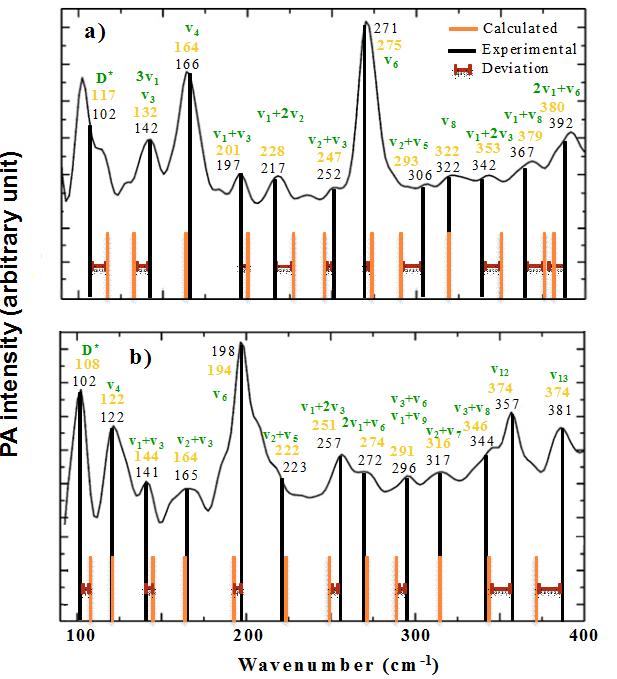
\includegraphics[scale=0.8]{image/final-exp}
 	\caption[Final assignment of the experimental infrared transitions for tetracene and pentacene]{Final assignment of the experimental infrared transitions for a) tetracene and b) pentacene. Calculated wavenumbers are indicated on the spectra with orange lines, and corresponding values above. Experimental values are indicated for comparison, and represented with dark lines}
 \end{figure}
 
 
 \begin{table}[htb]
 	\caption{Calculated intermolecular vibrational modes (cm$^{-1}$) and their intensities for distorted dimers of naphthalene, anthracene and tetracene.}
 	\begin{center}
 		\begin{tabular}{c c c c}
 			\toprule
 			\textbf{Type*} & \textbf{Naphthalene} & \textbf{Anthracene} & \textbf{Tetracene}\\
 			\midrule 
 			Translation 1/2 & 12(0.015) & 11(0.004) & 6(0) \\
 			Rotation 1/2 & 32(0.04) & 21(0.004) & 13(0.004)\\
 			Translation 1/2 & 47(0.007) & 33(0.002) & 21(0.005)\\
 			Rotation + Translation & 60(0.006) & 41(0.009) & 33(0.003)\\
 			\multicolumn{1}{p{4cm}}{\centering Translation \\ (remoteness of molecules)} & 73(0.008) & 55(0.01) & 46(0.2)\\
 			Rotation 1/2 & 94(0.14) & 73(0.2) &  \\
 			\multicolumn{1}{p{4cm}}{\centering Twisting of \\ the full system} &  &  & 
 			74(0.08)\\
 			\bottomrule
 			\end{tabular}
 	\end{center}
 	\footnotemark{* 1/2 means one molecule relative to the other.}
 \end{table}
 
 \section{Normal Vibrational Modes in Crystals}
 
 \subsection{Basic theory}
 
 The behavior of a system of interacting electrons  and nuclei is determined by the solutions of the time-dependent Schrödinger equation:
 
 where is the potential describing the coulombian interactions. The Born-Oppenheimer (or adiabatic) approximation (valid for ) allows to split the problem into an electronic problem depending upon nuclear positions :
 
 where and 
 
 
 \textsc{i.e.}
 
 and a nuclear problem under an effective interatomic potential determined by the electrons:
 
 determines the Potential Energy Surface and the equilibrium geometry. At equilibrium, forces on nuclei vanish:
 
 \textbf{Harmonic approximation}: the interatomic potential energy is expended to 2nd order. The resulting Hamiltonian transform into a sum of independent oscillators.
 
 Normal mode frequencies, and displacement patterns,  for Cartesian component  of atom, at atomic position  are determined by secular equation:
 
 where is the matrix of inter-atomic force constants, i.e. second derivatives of the energy with respect to atomic positions:
 
 In crystal, normal modes are classified by a wave-vector . Phonon frequencies, , and displacement patterns, , are determined by the secular equations:
 
 Introduce monochromatic perturbation to atomic positions as
 
 where represents the lattice vector and the equilibrium position of the -th atom in the unit cell.
 Fourier transform of force constants at  are second derivatives of the energy with respect to such monochromatic perturbations:
 
 \subsection{Results and discussion}
 
 We performed first-principle calculations for tetracene in order to clarify its structural and electronic properties of the solid-state system. These calculations strongly suggest the necessity to go beyond the standard DFT approach. First, we have shown that dispersion corrected methods are necessary to provide an improvement in the calculated lattice parameters and volume of the unit cell to compare with experimental values. The complete list of resulting lattice parameters, angles, and volumes along with experimental results for all the compounds are presented in Table 13. Furthermore, the mean absolute deviations observed for the calculation of these parameters for all the methods under consideration depend on the type of dispersion correction, and the relative errors on structural properties calculated using each method, in particular concerning the volume, may vary significantly. As mentioned by Lebegue et al \cite{appalakondaiah2015dispersion}, it has been demonstrated that one has to test all the dispersion corrected DFT methods for the C-, H-, N- and O- based energetic solids before concluding the ground state properties. In the present work, we show that the situation is the same for the S-based energetic solids. Since the D3 correction yields the most accurate structural descriptions of this model system, it has been used to calculate the vibrational, structural and electronic properties.
 
 \begin{table}[htb]
 	\caption{Lattice parameters of Tetracene molecule calculated in VASP code}
 	\begin{center}
 		\begin{tabular}{c c c c c c c}
 			\toprule
 			 & \textbf{D2} & \textbf{D3} & \textbf{TS} & \textbf{TS-SCS} & \textbf{PBE*} & \textbf{Exp} \\
 			 \midrule
 			 \textbf{a} &7.54 (7.41) &  7.92 & 7.71 & 7.70 & 9.25 & 7.90\\
 			 \textbf{b}& 5.96 (5.83) & 6.00 & 5.99 & 6.08 & 7.21 & 6.03 \\
 			 \textbf{c}& 13.28 (13.39) & 13.38 & 13.38 & 13.47 & 16.62 & 13.53 \\
 			 \textbf{$\alpha$} & 102.10 (102.21) & 101.21 & 101.36 & 100.97 & 101.36 &100.30\\
 			 \textbf{$\beta$} & 114.33 (113.23) & 113.26 & 113.61 & 114.39 & 112.14 & 113.20\\
 			 \textbf{$\gamma$} &85.20 (85.11) & 85.89 & 85.74 & 85.68 & 86.67 & 86.30\\
 			 \textbf{Volumen ($\AA^{3}$)} & 531.41 (519.01) & 572.96 & 554.74 &  563.74 & 1007.16 & 582.85\\
 			 \bottomrule
 		\end{tabular}
 	\end{center}
 	\footnotemark{PBE*: without dispersion correction}
 	\footnotemark{Parenthesis values were calculated with CRYSTAL program}
 \end{table}
 
 \begin{figure}[h]
 	\centering
 	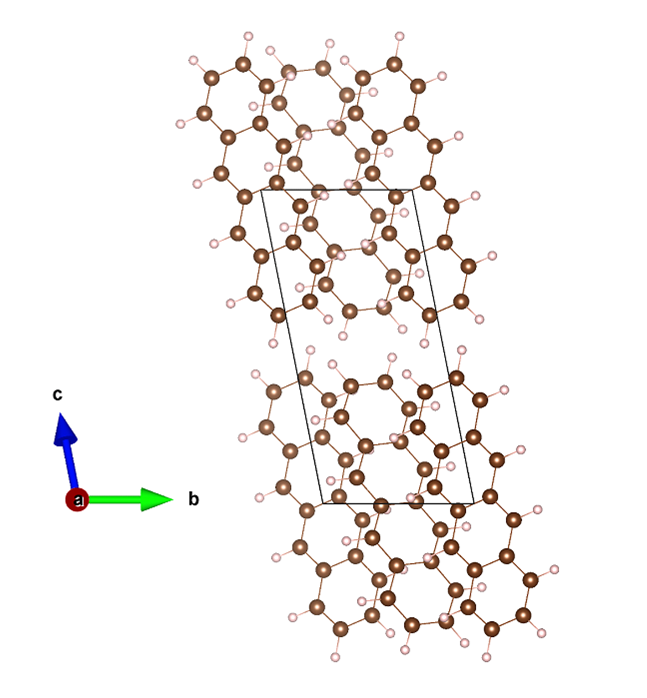
\includegraphics[scale=0.7]{image/T-a}
 \end{figure}
 
 \begin{figure}[h]
 	\centering
 	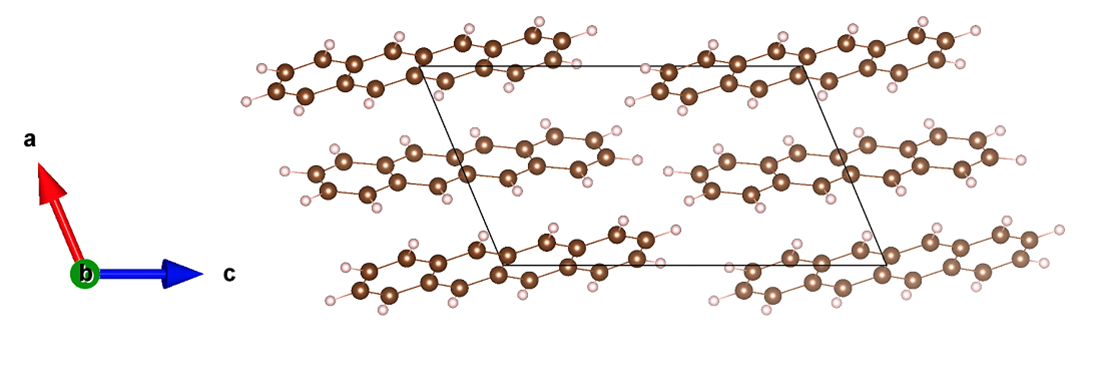
\includegraphics[scale=0.7]{image/T-b}
 \end{figure}
 
 \begin{figure}[h]
 	\centering
 	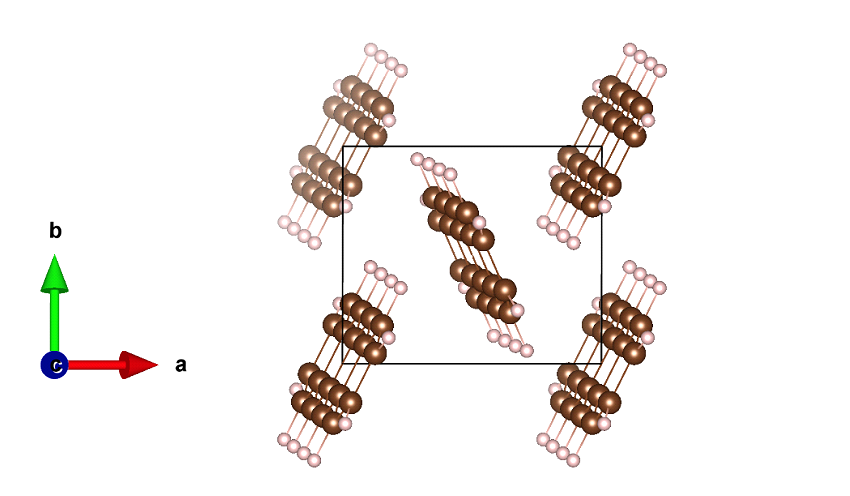
\includegraphics[scale=0.7]{image/T-c}
 \end{figure}
 
 Table 14 reports all the results obtained for tetracene, from the isolated up to the solid-state system. Beyond the numerical differences due to the various Hamiltonians used for these calculations, the results show significant differences on both vibration frequencies and intensities that are to be attributed to the effect of the chemical environment. Indeed, the signatures of some particular modes (such as $\nu_{2}$, $\nu_{8}$ and $\nu_{10}$) are modified with respect to the isolated system due to intermolecular interactions. Besides, our previous study on tetracene dimers revealed that intermolecular interactions induced the appearance of some characteristic spectral signatures at very low wavenumbers. For instance, the mode experimentally found at 106 cm$^{-1}$, which has been assigned, with aid of calculations, to a libration mode, is part of the characteristic signatures of intermolecular vibrations of acenes; the same mode was also assigned at 102 cm$^{-1}$ for the pentacene system. In fact, this mode cannot be only associated to a dimer: it results from the vibrations of the whole tetracene molecules within the network that constitutes the aggregate or the cristalline system. Our VASP calculations clearly show that this vibration mode is linked to distortions ofthe  crystalline network, which can be seen as the « breathing » of the network. Such a deformation was already partially taken into account in the study of a dimer. Some other modes of the crystalline network constitute, to a lesser extent, the remaining characteristic signatures of the intermolecular vibrations. More difficult to detect experimentally, these modes are theoretically found at 69.7 cm$^{1}$ ($\nu_{1}$), 128.5 c$^{-1}$ ($\nu_{3}$) and 320.8-323.8 cm$^{-1}$ ($\nu_{8}$). Unfortunately, there is no experimental data available below 100 cm$^{-1}$ for the tetracene system. But it seems that the $\nu_{3}$ and $\nu_{8}$ modes can now be identified as the modes of medium intensity reported from experimental data at 142 and 322 cm$^{-1}$, respectively. No fundamental mode nor combination mode of the isolated tetracene can be associated with the presence of those new experimental signatures.
 
 From all the modes calculated below 400 cm$^{-1}$, whatever their intensities are, they do not seem to be coupled to the vibration of the crystalline network. It suggests that calculations of the isolated molecule (or its dimer) are a sufficient approximation to identify these vibration modes. In the present case, it explains the fact that no assignation problem was found for regions beyond 150 cm$^{-1}$ during the molecular study of tetracene and its dimer. At the molecular level, calculations on small aggregates can be sufficient to identify the modes of the crystalline network that are significantly impacted. 
 
 To conclude, the use of a model able to describe the chemical environment was essential to identify the spectral signatures of the inter-molecular modes that we try to characterize in our study of asphaltenes (or, at least, of acenes systems). The calculated phonon spectrum thus seems to answers, even if our calculations up to now do not account for both mechanical and electrical anharmonicities. Such conditions are all the more necessary for an exhaustive study of the modes of each isolated molecule. Particularly, it allows an identification of the combination modes as well as the harmonics for which the signatures have been clearly evidenced by photo-acoustic measurements. Only a double approach (both molecular and solid-state) can allow one to completely identify the photo-acoustic results of acenes molecules in the crystalline state.
 
 \begin{table}[htb]
 	\caption{ Calculated vibrational frequencies (cm$^{-1}$) of the monomer, dimer and solid-state (PBE tetracene system.}
 	\begin{center}
 		\begin{tabular}{c c c c c}
 			\toprule
 			\multicolumn{2}{p{4.5cm}}{\centering \textbf{Monomer}} & \textbf{Dimer} & \multicolumn{1}{p{4cm}}{\centering \textbf{Experimental} \\ \textbf{(P.A.) this work}} & \textbf{VASP/CRYSTAL}\\
 			Assignment & $\nu$(cm$^{-1}$) & $\nu$(cm$^{-1}$) & $\nu$(cm$^{-1}$) & $\omega$(cm$^{-1}$) \\
 			& Int(km/mol) & Int(km/mol) & & Int(relative) \\
 			\midrule
 			& & \textit{15 (<0.01)} & & \\
 			& & \textit{31 (0)} & & \\
 			& & \textit{52 (0)} & & \\
 		   $\nu_{1}$& 57 (0.8) & 59 (0.6) &  & 69.7 (8.2) \\
 		   & & \textit{80 (1.0)} & & \\
 		   & & \textit{87 (0.1)} & & \\
 		  & & 94 (0) & & \\
 		  & & 112 (0) & & \\
 		  $\nu_{2}$ & 93 (0) & 117 (0.3) & 106 (m) + sh & \multicolumn{1}{p{4cm}}{\centering 102.4 (2.1) \\ 105.7 (9.5)}\\
 		  & & 124 (0) & & \\
 		  3$\nu_{1}$& 132 (<0.01) & & & \\
 		  $\nu_{3}$& 153 (0.01) &  & 142 (m) & \multicolumn{1}{p{4cm}}{\centering 128.5 (7.1) \\ 148 (0.1)}\\ 
 		  & & 162 (0)&  & \\
 		  $\nu_{4}$& 164 (1.3) & 168 (1.7) & 166 (s) + sh & 164.6 (15.5) \\
 		  & & 169 (0) & & \\
 		  $\nu_{5}$ & 196 (0.05) & 176 (0.2) & 197 (w) & 170.1 (0.1) \\
 		  $\nu_{1}+\nu_{3}$ & 201 (<0.01) &  &  & \\
 		  & & 208 (0) & & \\
 		  &  & 212 (0.09) & 217 (w) & \\
 		  $\nu_{1}+ 2\nu_{2}$ & 228 (<0.01) & & & \\
 		  $\nu_{2}+\nu_{3}$& 247 (0.01) &  & 252 (vw) & \\
 		  $\nu_{6}$ & 275 (1.03) & 282 (1.6) & 271 (m) & 267.4 (3.0)\\
 		  	&  & 286 (0) &  & 274.6 (2.6)\\
 		  	$\nu_{2}+ \nu_{5}$ & 293 (<0.01) &  & 306 (vw) & \\
 		  	& & 316 (0) & & \\
 		   & & 316 (0.03) & & \\
 		    &  & 324 (0) & 322 (w) & 320.8 (0.9)\\
 		    $\nu_{8}$& 322 (<0.01) & 325 (0.06) & & 323.8 (0.5)\\
 		    &  & 335 (0.03) & 342 (w) & \\
 		    & & 335 (0) & & \\
 		    $\nu_{1}+ 2\nu_{3}$ & 353 (<0.01) & &  & \\	
 		    $\nu_{1}+ \nu_{8}$ & 379 (<0.01) & & & \\
 		    $\nu_{10}$ & 385 (0.04) & 390 (0.02) &  392 (m) & \\
 		    2$\nu_{1}+ \nu_{6}$ & 380 (<0.01) &  & & \\
 		    \bottomrule	    
 		  \end{tabular}
 	\end{center}
 	\footnotemark[1]{italic: Intermolecular modes}
 \end{table}
 
 \section*{Conclusions}
 
 The DFT calculations presented in this work provide detailed and accurate descriptions of experimental photoacoustic far IR spectra for tetracene and pentacene and for far IR spectra of the acene family as a whole.  The impacts of molecular distortion on monomer and dimer spectra and dimer stability, and the interpretation of peaks in photoacoustic IR spectra of crystalline solids are discussed in detail. Distortion breaks molecular symmetry and this adds to the complexity of the interpretation of the resulting spectra. Inter- and intramolecular vibrations in the acene family of compounds are discriminated, and combinations of inter- and intramolecular vibrations are identified specially with the use od solid-state conditions. Peak assignment ambiguity, and the potential impacts of molecular distortion on peak intensity are addressed for tetracene and pentacene. By examining computed and experimental spectra for the family of acene molecules concurrently, trends in vibration modes with molecular size were used to reinforce assignments, and to reattribute assignments made previously in the experimental tetracene and pentacene spectra. In particular, both dimer and solid state calculations permitted re-assignment of an infrared active peak arising in tetracene at 142 cm$^{-1}$ and assignment of large infrared active peaks at 117 and 108 cm$^{-1}$ for tetracene and pentacene respectively that may permit their identification in an acene mixture. The intermolecular vibrations for naphthalene, anthracene, tetracene and pentacene, are found in the same wavelength range of the far infrared spectrum and are not readily discriminated one from the other. The specificity of the acene $\pi$-stacking interactions, reinforced by calculations with distorted dimers (and solid-state), allows not only the identification of this family of molecules, but also highlights the presence of $\pi$-stacking interaction in a mixture as a whole.
 
 \newpage
 
 \section*{Supplementary Data}
 
 \begin{figure}[h]
 	\centering
 	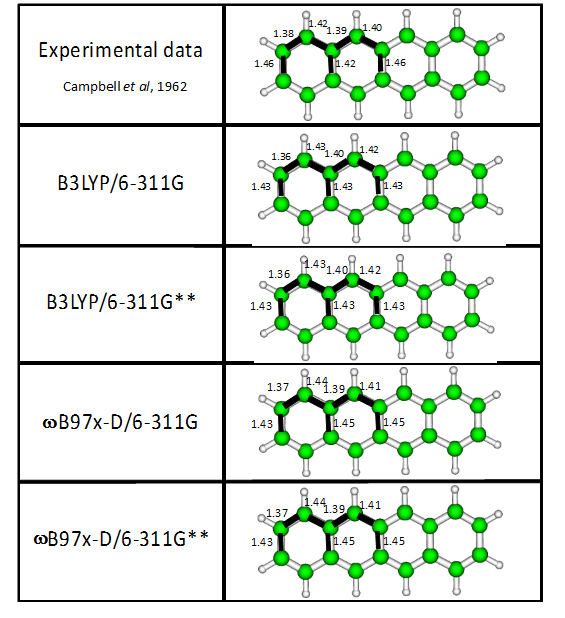
\includegraphics[scale=0.8]{image/geometrical-data}
 	\caption[Geometrical data for a tetracene molecule]{Geometrical data for a tetracene molecule by Campbell et al \cite{campbell1962crystal} and values optimized in the framework of various DFT calculations, used in this work}
 \end{figure}
 
 \begin{figure}[h]
 	\centering
 	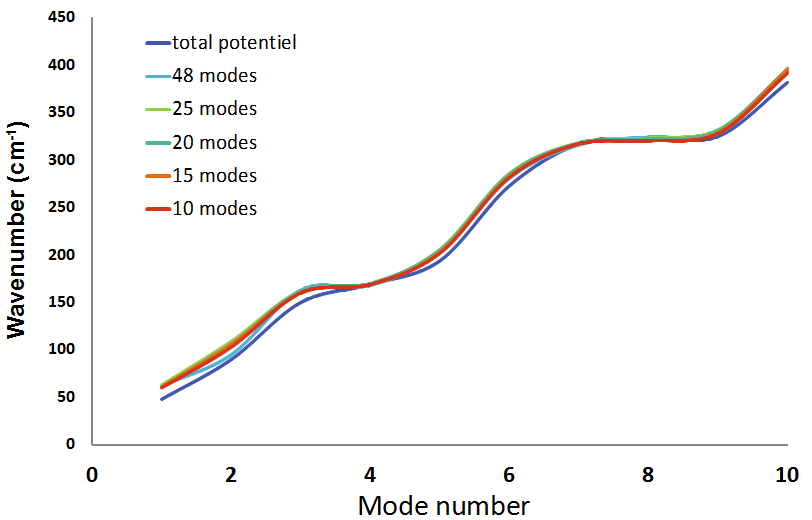
\includegraphics[scale=0.8]{image/mode-trunc}
 	\caption[Effect of mode truncature on the first ten mode on wavenumber of tetracene ]{Effect of mode truncature on the wavenumber obtained using $\omega$B97X-D/6-311G for the first ten vibration modes of a tetracene molecule, with force truncature (f>5cm$^{-1}$)}
 \end{figure}
 
 \begin{table}
 	\caption{Computed wavenumbers and intensities for distorted tetracene based on the harmonic approximation at the $\omega$B97X-D/6-311G level of calculation. Comparison with symmetric tetracene (D$_{2h}$)}
 	\begin{center}
 		\begin{tabular}{c c c c c}
 			\toprule
 			& \multicolumn{2}{p{8cm}}{\centering \textbf{Tetracene with D$_{2h}$ symmetry}} & \multicolumn{2}{p{8cm}}{\centering \textbf{Distorted Tetracene}}\\
 			Mode & \multicolumn{1}{p{4cm}}{\centering Harmonic \\ wavenumber (cm$^{-1}$)} & \multicolumn{1}{p{3.5cm}}{\centering Harmonic Intensity \\ (km.mol$^{-1}$)}& \multicolumn{1}{p{4cm}}{\centering Harmonic \\ wavenumber (cm$^{-1}$)} & \multicolumn{1}{p{3.5cm}}{\centering Harmonic Intensity \\ (km.mol$^{-1}$)}\\
 			\midrule
 			$\nu_{1}$ & 57 & 0.86 & 58 & 0.87 \\
 			$\nu_{2}$ & 93 & 0 & 93 & 0.03 \\
 		   $\nu_{3}$ & 154 & 0 & 154 & 0.01\\
 		   $\nu_{4}$ & 168 & 1.24 & 168 & 1.22\\
 		   	$\nu_{5}$ & 196 & 0 & 197 & 0.05\\
 		   	$\nu_{6}$ & 276 & 1.03 & 277 & 1.06\\
 		   	$\nu_{7}$& 316 & 0 & 316 & 0.002\\
 		   	$\nu_{8}$& 324 & 0 & 324 & 0.002\\
 		   	$\nu_{9}$& 328 & 0 & 328 & 0.02\\
 		   	$\nu_{10}$& 389 & 0 & 389 & 0.04\\
 		   				\bottomrule
 		\end{tabular}
 	\end{center}
 \end{table}
 

\begin{table}[htb]
	\caption{Calculated and Experimental wavenumbers (cm-1)\cite{boys1970calculation} of the vibrational modes of a naphthalene molecule. Values in parenthesis represent the deviation between the calculated and experimental wavenumbers.}
	\begin{center}
		\begin{tabular}{c c c c c c c c}
		\toprule
		\textbf{Mode} & \textbf{Symmetry} & \multicolumn{2}{p{3.4cm}}{\textbf{B3LYP/6-311G}} & \multicolumn{2}{p{3.7cm}}{\textbf{$\omega$B97X-D/6-311G}} & \textbf{Saeki et al\cite{saeki2006theoretical}} & \textbf{Exp\cite{gonzalez2000quantum}}\\
		\midrule
		&  & Harmonic & PT2 & Harmonic & PT2 &  & \\
		\cline{3-6}
		$\nu_{32}$& b$_{1g}$ &	177(+1) & 176(0) & 177(+1) & 176(0) & 168(-8) & 176\\
		$\nu_{28}$ & a$_{1u}$ & 189(-6) & 186(-9) & 190(-5) & 187(-8) & 182(-13) & 195\\
		$\nu_{40}$ & b$_{3u}$ & 373(+14) & 372(+13) & 379(+20) & 377(+18) & 356(-3) & 359\\
		$\nu_{20}$ & b$_{1u}$ & 401(+15) & 394(+8) & 404(+18) & 398(+12) & 377(-9) & 386\\
		\bottomrule				
		\end{tabular}
\end{center}
\end{table}


 
 \begin{table}[htb]
 	\caption{Intramolecular vibration modes (cm$^{-1}$) and the corresponding intensities in brackets (km/mol) for distorted naphthalene, anthracene and tetracene dimers. Values of corresponding dimer modes of molecules in D$_{2h}$ configuration are written below in italics.}
 	\centering    
 	\begin{tabular}{c|c c c}
 		\hline 		
 		\textbf{Type} & \textbf{Naphthalene} & \textbf{Anthracene} & \textbf{Tetracene}\\
 		\hline
 		\multicolumn{1}{p{3cm}|}{Butterfly sw} & \multicolumn{1}{p{3cm}}{\centering 190(8.8) \\
 			\textit{188(3.8)}} & \multicolumn{1}{p{3.5cm}}{\centering 101(0.003) \\
 			\textit{111(0.8)/112(1.2)}} & \multicolumn{1}{p{3cm}}{\centering 77(1.6) \\
 			\textit{59(0.6)}}\\
 		\multicolumn{1}{p{3cm}|}{Butterfly ow} & \multicolumn{1}{p{3cm}}{\centering 183(0.03) \\
 			\textit{196(0)}} & \multicolumn{1}{p{3.5cm}}{\centering 103(4.2) \\
 			\textit{128(0)}} & \multicolumn{1}{p{3cm}}{\centering 54(0.005) \\
 			\textit{94(0)}}\\
 		\multicolumn{1}{p{3cm}|}{Twisting sw} & \multicolumn{1}{p{3cm}}{\centering 206(0.2) \\
 			\textit{207(1.2)}} & \multicolumn{1}{p{3.5cm}}{\centering 137(0.05) \\
 			\textit{148(0.6)}} & \multicolumn{1}{p{3cm}}{\centering 106(0.4) \\
 			\textit{117(0.3)}}\\
 		\multicolumn{1}{p{3cm}|}{Twisting ow} & \multicolumn{1}{p{3cm}}{\centering 208(0.06) \\
 			\textit{208(0)}} & \multicolumn{1}{p{3.5cm}}{\centering 141(0.005) \\
 			\textit{149(0.02)}} & \multicolumn{1}{p{3cm}}{\centering 102(0.04) \\
 			\textit{124(0)}}\\
 		\multicolumn{1}{p{3cm}|}{Scissoring sw} & \multicolumn{1}{p{3cm}}{\centering 382(2.1) \\
 			\textit{381(2.2)}} & \multicolumn{1}{p{3.5cm}}{\centering 244(1.9) \\
 			\textit{244(2.05)}} & \multicolumn{1}{p{3cm}}{\centering 168(1.8) \\
 			\textit{168(1.7)}}\\
 		\multicolumn{1}{p{3cm}|}{Scissoring ow} & \multicolumn{1}{p{3cm}}{\centering 382(0.2) \\
 			\textit{380(0)}} & \multicolumn{1}{p{3.5cm}}{\centering 243(0.2) \\
 			\textit{243(0)}} & \multicolumn{1}{p{3cm}}{\centering 168(0.1) \\
 			\textit{169(0)}}\\
 			\multicolumn{1}{p{3cm}|}{Wagging sw} & \multicolumn{1}{p{3cm}}{\centering 411(1.9) \\
 				\textit{405(0)}} & \multicolumn{1}{p{3.5cm}}{\centering 251(0.3) \\
 				\textit{250(0)}} & \multicolumn{1}{p{3cm}}{\centering 164(0.03) \\
 				\textit{162(0)}}\\
 		\multicolumn{1}{p{3cm}|}{Wagging ow} & \multicolumn{1}{p{3cm}}{\centering 410(0.03) \\
 			\textit{405(0.02)}} & \multicolumn{1}{p{3.5cm}}{\centering 248(0.2) \\
 			\textit{253(0.17)}} & \multicolumn{1}{p{3cm}}{\centering 154(0.1) \\
 			\textit{176(0.2)}}\\
 			\multicolumn{1}{p{3cm}|}{Twisting sw} & \multicolumn{1}{p{3cm}}{\centering 502(0.1) \\
 				\textit{498(0)}} & \multicolumn{1}{p{3.5cm}}{\centering 282(0.05) \\
 				\textit{285(0.02)}} & \multicolumn{1}{p{3cm}}{\centering 203(0.03) \\
 				\textit{208(0)}}\\
 		\multicolumn{1}{p{3cm}|}{Twisting ow} & \multicolumn{1}{p{3cm}}{\centering 503(0.3) \\
 					\textit{499(15.2)}} & \multicolumn{1}{p{3.5cm}}{\centering 281(0.003) \\
 					\textit{286(0.08)}} & \multicolumn{1}{p{3cm}}{\centering 201(0.2) \\
 					\textit{212(0.09)}}\\	
 		\multicolumn{1}{p{3cm}|}{Wagging sw} & \multicolumn{1}{p{3cm}}{\centering 492(59) \\
 			\textit{504(45.0)}} & \multicolumn{1}{p{3.5cm}}{\centering 400(0.01) \\
 			\textit{396(0.2)}} & \multicolumn{1}{p{3cm}}{\centering 281(2.2) \\
 			\textit{282(1.55)}}\\		
 		\multicolumn{1}{p{3cm}|}{Wagging ow} & \multicolumn{1}{p{3cm}}{\centering 495(1.2) \\
 			\textit{507(0)}} & \multicolumn{1}{p{3.5cm}}{\centering 398(0.01) \\
 			\textit{396(0.04)}} & \multicolumn{1}{p{3cm}}{\centering 279(0.2) \\
 			\textit{286(0)}}\\	
 		\multicolumn{1}{p{3cm}|}{Stretching sw} & \multicolumn{1}{p{3cm}}{\centering 533(0.02) \\
 			\textit{534(0)}} & \multicolumn{1}{p{3.5cm}}{\centering 407(0.007) \\
 			\textit{407(0)}} & \multicolumn{1}{p{3cm}}{\centering 324(0.007) \\
 			\textit{324(0)}}\\	
 		\multicolumn{1}{p{3cm}|}{Stretching ow} & \multicolumn{1}{p{3cm}}{\centering 532(0.01) \\
 			\textit{534(0.09)}} & \multicolumn{1}{p{3.5cm}}{\centering 407(0.02) \\
 			\textit{407(0.04)}} & \multicolumn{1}{p{3cm}}{\centering 324(0.07) \\
 			\textit{325(0.06)}}\\
 		\multicolumn{1}{p{3cm}|}{Rocking sw} & \multicolumn{1}{p{3cm}}{\centering 536(0.1)/536(0.2)$^{1}$ \\
 			\textit{537(0)}} & \multicolumn{1}{p{3.5cm}}{\centering 413(0.03) \\
 			\textit{412(0)}} & \multicolumn{1}{p{3cm}}{\centering 316(0.01)/316(0.004)$^{1}$ \\
 			\textit{316(0)}}\\
 		\multicolumn{1}{p{3cm}|}{Rocking ow} & \multicolumn{1}{p{3cm}}{\centering 536(0.1)/536(0.2)$^{1}$ \\
 			\textit{537(0.06)}} & \multicolumn{1}{p{3.5cm}}{\centering 413(0.009) \\
 			\textit{412(0.01)}} & \multicolumn{1}{p{3cm}}{\centering 316(0.01)/316(0.004)$^{1}$ \\
 			\textit{316(0.03)}}\\
 		\multicolumn{1}{p{3cm}|}{Twisting sw} & \multicolumn{1}{p{3cm}}{\centering 660(0.06) \\
 			\textit{658(0.4)}} &  & \multicolumn{1}{p{3cm}}{\centering 331(0.03)/331(0.02)$^{1}$ \\
 			\textit{335(0.03)}}\\
 		\multicolumn{1}{p{3cm}|}{Twisting ow} & \multicolumn{1}{p{3cm}}{\centering 660(0.007) \\
 			\textit{659(0)}} &  & \multicolumn{1}{p{3cm}}{\centering 331(0.03)/331(0.02)$^{1}$ \\
 			\textit{336(0)}}\\
 		\multicolumn{1}{p{3cm}|}{Wagging sw} &  & \multicolumn{1}{p{3.5cm}}{\centering 487(66.8) \\
 			\textit{496(70.5)}} & \multicolumn{1}{p{3cm}}{\centering 389(0.02) \\
 			\textit{390(0)}}\\
 		\multicolumn{1}{p{3cm}|}{Wagging ow} &  & \multicolumn{1}{p{3.5cm}}{\centering 490(1.07) \\
 			\textit{497(0.5)}} & \multicolumn{1}{p{3cm}}{\centering 389(0.02) \\
 			\textit{390(0.02)}}\\
 		\hline
 	\end{tabular}\\
 	\begin{flushleft}
 	\footnotemark[1]{The vibrational modes for which two values are indicated correspond to modes for which one molecule vibrates at a time}	
 	\end{flushleft}
 	\label{A33}
 \end{table}